%%%%%%%% ICML 2026 PAPER DRAFT %%%%%%%%%%%%%%%%%

\documentclass{article}

\usepackage{microtype}
\usepackage{graphicx}
\usepackage{subcaption}
\usepackage{booktabs}
\usepackage{hyperref}
\newcommand{\theHalgorithm}{\arabic{algorithm}}
\usepackage[preprint]{icml2026}
\usepackage{amsmath}
\usepackage{amssymb}
\usepackage{mathtools}
\usepackage{amsthm}
\usepackage[capitalize,noabbrev]{cleveref}
\usepackage{listings}
\lstset{
  basicstyle=\ttfamily\scriptsize,
  breaklines=true,
  breakatwhitespace=false,
  columns=fullflexible,
  keepspaces=true,
  showstringspaces=false,
  literate={—}{{--}}1
}

\icmltitlerunning{\smash{Evidence-Bound Review Agents}}

\begin{document}

\twocolumn[
  \icmltitle{Optimizing Evidence-Bound Review Agents with\\
    Consolidated Human Peer Reviews}

  \icmlsetsymbol{equal}{*}
  \begin{icmlauthorlist}
    \icmlauthor{Seongsu Bae}{equal,kaist}
    \icmlauthor{Kyunghoon Hur}{equal,keti}
    \icmlauthor{Gyubok Lee}{equal,kaist}
  \end{icmlauthorlist}

  \icmlaffiliation{kaist}{KAIST}
  \icmlaffiliation{keti}{Korea Electronics Technology Institute (KETI)}
  \icmlkeywords{scientific peer review, review agents, pseudo-labeling, automated research}
  \vskip 0.3in
]

\printAffiliationsAndNotice{\icmlEqualContribution}

\begin{abstract}
AI agents increasingly automate experimentation and scientific writing, creating a corresponding need for scalable and reliable evaluation. Existing LLM reviewers are commonly prompted directly or evaluated against individual reviews, although reviews of the same paper can be inconsistent, complementary, or uneven in quality. From 6,341 accepted ICML 2026 papers, we draw a 600-paper stratified sample and construct consolidated pseudo-labels for an initial subset of 175 papers. We implement a label-blind review agent that reads PDF-derived manuscript text, produces an evidence trace and rubric-specific rationales, and returns schema-validated ICML scores. On a fixed five-paper development smoke test, prompt calibration increases the development objective from 0.895 to 0.947 and is selected by predefined non-regression gates. These preliminary results establish operational feasibility, not performance on unseen papers or parity with human reviewers.
\end{abstract}

\section{Introduction}

Scientific agents are beginning to support increasingly large portions of the research lifecycle, including idea generation, coding, experimentation, analysis, and manuscript writing. Systems such as The AI Scientist and Agent Laboratory demonstrate end-to-end workflows that produce complete research artifacts with limited human intervention \cite{lu2024aiscientist,schmidgall2025agentlab}. AutoResearch-style systems further increase the rate at which experimental candidates can be generated and evaluated. As scientific generation becomes more scalable, scientific evaluation risks becoming a bottleneck.

Automated peer review is not simply a summarization or acceptance-prediction task. A useful reviewer must identify the main claims, connect them to evidence, distinguish soundness from significance and presentation, formulate actionable questions, and keep numerical scores consistent with the written assessment. Directly prompted LLMs can produce fluent reviews, but fluency does not guarantee specific or supported criticism. Recent work therefore explores reasoning models and proactive reviewer agents that maintain explicit review evidence \cite{zhang2025critical,fang2026proreviewer}.

Human review data also presents a supervision problem. Reviews of the same paper often emphasize different aspects and assign different scores. Treating every review as an independent target exposes a model to conflicting supervision, while choosing one review discards complementary observations. Moreover, some reviews may be cursory or insufficiently grounded. We therefore study the following question: \emph{How can multiple, partially inconsistent human reviews be converted into coherent supervision for a scientific review agent?}

We build a paper-level dataset that links multiple initial reviews, rubric scores, and a meta-review, and use an LLM-based procedure to consolidate them into one ICML-style pseudo-review. The procedure is a quality-control mechanism, not a claim of objective ground truth: it asks the labeling model to prioritize specific, mutually corroborated concerns, remove duplication, and write from a single-reviewer perspective. It also restricts each synthesized score to the minimum--maximum range of the corresponding human scores.

Our contributions are:
\begin{itemize}
  \item a distribution-matched sample of 600 papers, stratified from 6,341 accepted papers by research area and review-score quartile;
  \item 175 consolidated pseudo-labels, including separate audit metadata for 163 labels and verified score-range compliance for all 175; and
  \item an end-to-end, manuscript-only review agent with strict structured output, bounded prompt optimization, and a reproducible preliminary development evaluation.
\end{itemize}

\section{Related Work}

\subsection{LLM-based Scientific Peer Review and Reviewer Agents}

Recent reviewer systems range from reasoning-based manuscript quality checkers to agents that actively investigate suspicious claims. The former focus on critical problems rather than imitating a complete human review \cite{zhang2025critical}; ProReviewer instead maintains a structured review log during evidence collection \cite{fang2026proreviewer}. Our work is complementary: we construct paper-level supervision from multiple reviews and optimize an evidence-bound structured reviewer against it.

\subsection{AutoResearch and AI-Generated Scientific Papers}

Research agents now automate literature exploration, hypothesis generation, experimental iteration, and paper writing. The AI Scientist generates ideas, executes experiments, writes a manuscript, and invokes an automated review stage \cite{lu2024aiscientist}; Agent Laboratory organizes literature review, experimentation, and report writing with optional human feedback \cite{schmidgall2025agentlab}. AutoResearch-style loops narrow this workflow to rapid, metric-driven modification and evaluation of experimental code \cite{karpathy2025autoresearch}. These systems motivate our setting: increasing the throughput of research generation also increases the need for independent, evidence-grounded evaluation. A reviewer agent should therefore complement generation systems rather than merely reproduce their self-evaluation.

\section{Dataset Construction}

\subsection{Source Records}

We group public ICML 2026 OpenReview records by paper forum identifier. The accepted-paper collection contains 6,341 papers and 24,378 official reviews. We sample 600 papers (9.5\%) using largest-remainder allocation over primary areas and, within each area, quartiles of mean reviewer overall recommendation (seed 42). The sample covers 81 of 84 areas; its mean score is 4.144 versus 4.147 in the population, and its spotlight share is 7.7\% versus 8.5\%. We generated consolidated labels for 175 sampled papers (166 regular and 9 spotlight).

Our input construction excludes explicit rebuttal and post-rebuttal score-change fields. A meta-review may nevertheless refer to the rebuttal or decision, so we prohibit such references in the synthesized review. The review agent receives only the manuscript at inference time; human reviews, meta-reviews, rebuttals, and decisions are unavailable to it.

Multiple reviews provide complementary expertise but do not form a consistent training target. Reviewers can focus on different contributions, disagree about severity, or assign substantially different scores. Review effort can also vary: a detailed, evidence-backed review and a cursory review should not necessarily influence a consolidated target equally. We use pseudo-labeling to reduce contradictions and duplication while retaining well-supported observations across reviews. This procedure cannot guarantee that the output is correct or unbiased; it is an auditable quality-control step for constructing supervision.

\subsection{Constrained Consolidation}

For each paper, the labeling model reads the initial reviews and the meta-review. It is prompted to assign each source review a qualitative priority (high, medium, or low) using specificity, cross-review corroboration, and agreement with concerns reflected in the meta-review. These priorities and their rationales are stored separately as labeling metadata. They are neither numerical reliability estimates nor included in the final review text.

The model then produces one review in the voice of a single reviewer. It may merge and rephrase supported observations, but it is instructed not to invent criticisms absent from the source reviews or mention reviewers, the meta-review, rebuttal, or decision. The final JSON contains exactly the ten review fields listed above; reviewer priorities and the score rationale are stored in a separate audit file.

For paper $i$, review dimension $d$, and human reviews $R_i$, the synthesized score $\hat{s}_{i,d}$ is constrained by
\begin{equation}
  \min_{r\in R_i}s_{r,d}\leq \hat{s}_{i,d}\leq\max_{r\in R_i}s_{r,d}.
\end{equation}
This constraint covers soundness, presentation, significance, originality, and overall recommendation. We checked all 175 current pseudo-labels and found no score-range violations. The constraint prevents extrapolation beyond observed judgments, but does not imply a true consensus score.

\section{Review Agent and Development Evaluation}

\begin{figure*}[t]
  \centering
  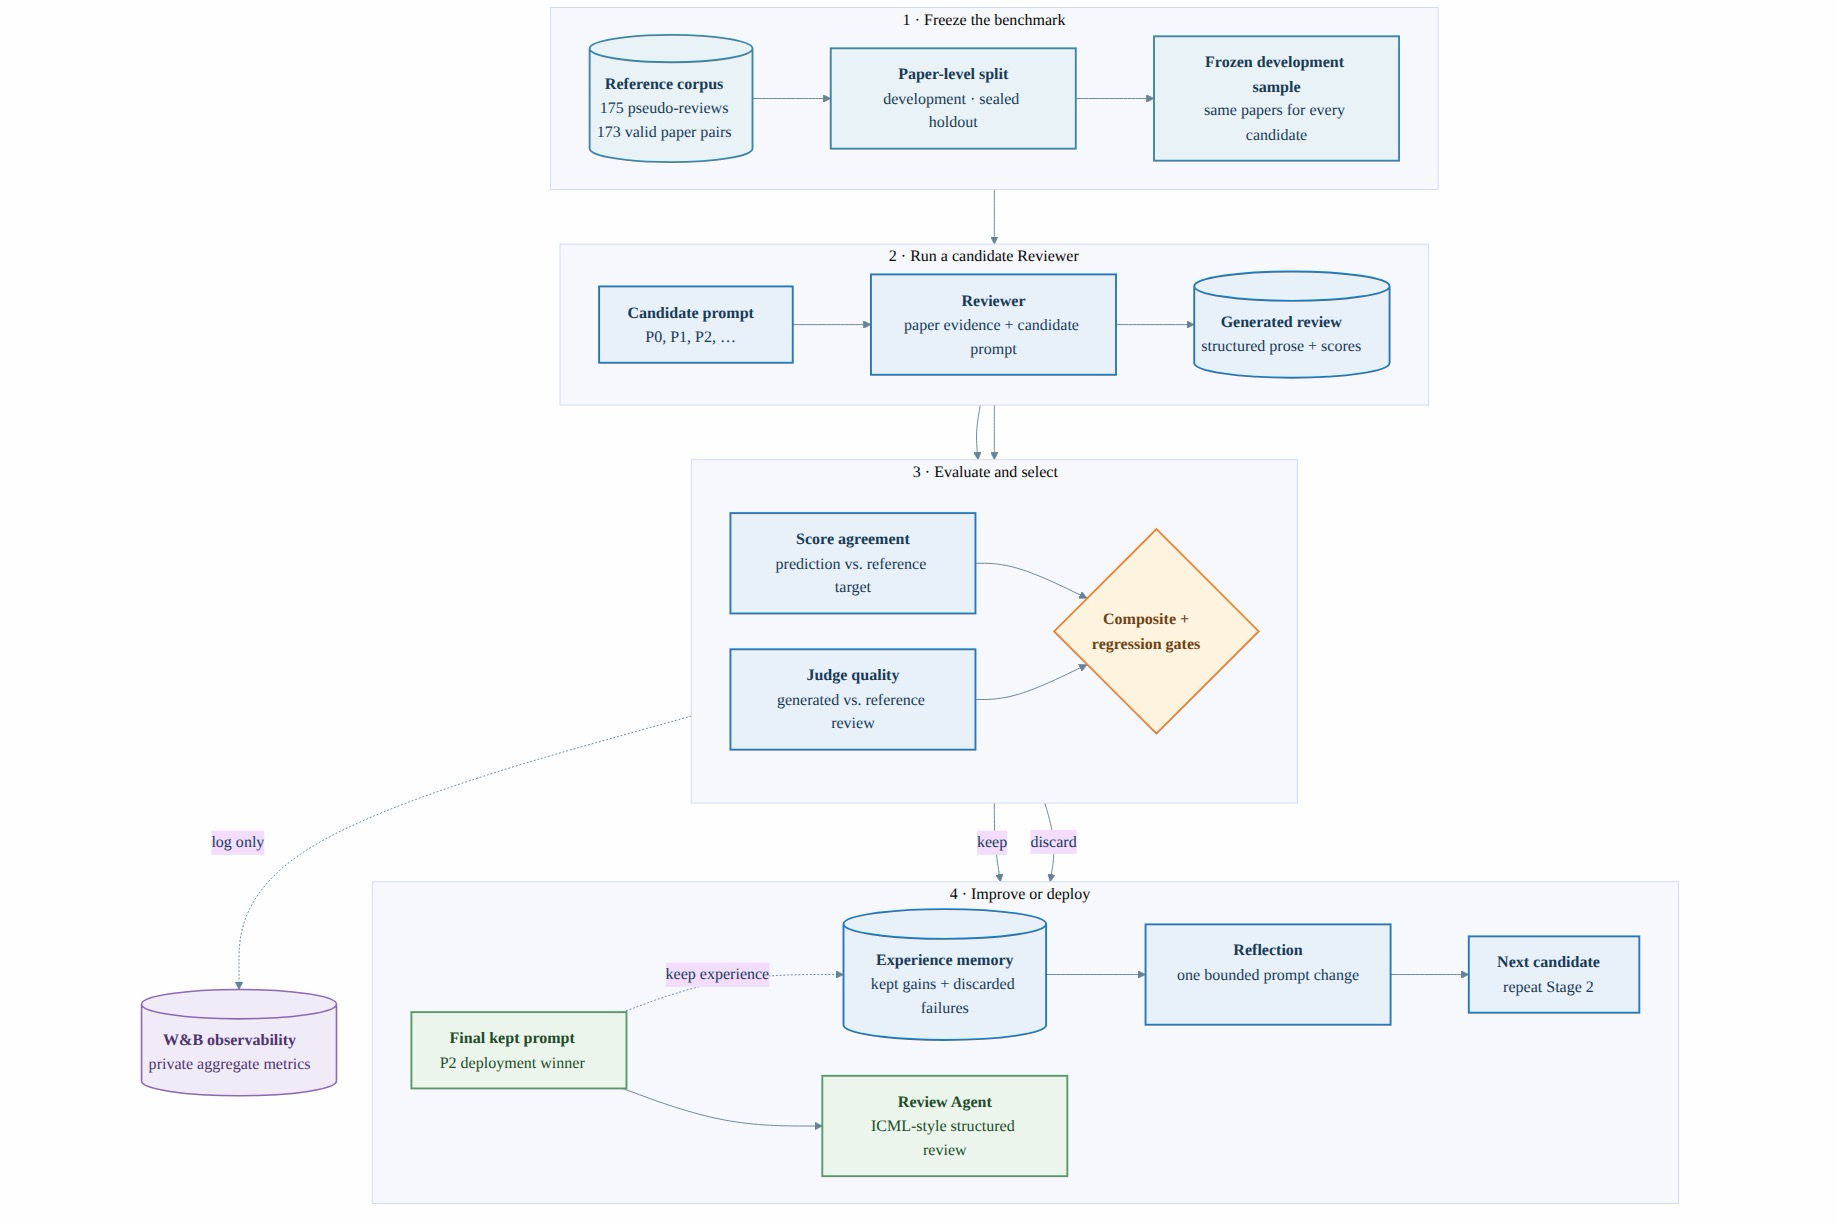
\includegraphics[width=0.90\textwidth]{../docs/figures/image.png}
  \caption{End-to-end review-agent development workflow. A frozen pseudo-review benchmark supports manuscript-only Reviewer inference, reference-score and Judge evaluation, regression-gated prompt selection, experience-guided reflection, and deployment of the kept P2 prompt.}
  \label{fig:system}
\end{figure*}

\paragraph{Manuscript-only reviewer.}
\Cref{fig:system} summarizes the implementation. The runner extracts text and metadata from a PDF, places the text in a delimited untrusted-data block, and invokes a no-tools reviewer through Codex authentication. Web search, external memory, and paper-embedded instructions are disabled. The selected P2 prompt asks GPT-5.4 to produce a descriptive summary, strengths, severity-ordered weaknesses, decision-relevant questions, limitations, ethical concerns, and an evidence trace. It also requires six ICML scores and paper-grounded rationales. A strict JSON schema and runtime validator reject unknown fields, missing prose, and out-of-range scores. During inference, the reviewer cannot access pseudo-label prose, reference scores, candidate identity, or Judge output.

\paragraph{Optimization objective.}
We optimize only the reviewer prompt on a frozen five-paper development sample. A separate GPT-5.4 Judge receives the manuscript, generated review, and reference pseudo-review prose, but not numeric reference scores or candidate identity. The local evaluator combines normalized agreement with consolidated pseudo-label scores ($A$), nine-dimension Judge quality ($J$), and penalties $P$ for hallucination, missing evidence, schema failure, and API failure:
\begin{equation}
  C=\operatorname{clip}_{[0,1]}(0.5A+0.5J-0.25P).
\end{equation}
A candidate is kept only if $C$ improves and neither aggregate component nor any score dimension crosses a predefined regression threshold. Discarded prompts are retained for analysis but cannot become the next optimization parent.

\paragraph{Development results.}
P2 adds an evidence-to-ordinal calibration pass and separates significance from soundness and originality. Relative to P0, it improves composite score by 0.051, reference-score agreement by 0.064, and Judge quality by 0.039, while passing every gate. All five papers completed with ten Reviewer/Judge calls and no retries or failures. P3 attains a slightly higher raw composite but is discarded because score agreement and dimension gates regress; P4 also fails to improve on P2. We therefore freeze P2 as the development default. Because this selection uses only five development papers, no holdout, and the same model version for Reviewer and Judge, it does not establish general review quality.

\section{Limitations}

The current pseudo-labeled subset is small and contains only accepted papers, limiting both score coverage and variation in manuscript quality. Although the 600-paper sample preserves the population's area and mean-score distributions, three very small areas receive no sample and the accepted-only population contains few low-score papers. Meta-reviews are not objective ground truth, and consolidation can suppress legitimate disagreement. The agent evaluation is a five-paper development smoke with no sealed-holdout result, uncertainty estimate, or human-expert comparison; using GPT-5.4 as both Reviewer and Judge also risks correlated preferences. Finally, rejected papers and their reviews can be difficult to collect because they may remain inaccessible unless authors voluntarily make them public. Publicly available rejected papers may therefore be an unrepresentative subset.

\section{Conclusion and Future Directions}

We introduced a data construction framework and operational review agent for evaluating scientific manuscripts against consolidated human-review supervision. The framework converts partially inconsistent reviews into an auditable pseudo-review, while the label-blind agent produces evidence-traced, schema-validated assessments. A bounded five-paper development campaign selects P2 over P0, but this result remains preliminary.

We will next evaluate the frozen P2 prompt once on a larger sealed holdout, report paired uncertainty, and conduct blinded human-expert comparisons with independent Judge models. On the data side, we will expand beyond 175 labels, strengthen stratification for rare areas and score tails, and incorporate voluntarily disclosed rejected papers while measuring availability-driven selection bias. These extensions are required before making claims about general ICML reviewing performance.

\bibliography{bibliography}
\bibliographystyle{icml2026}

\newpage
\appendix
\onecolumn

\section{Label-Construction Prompt}
We use the version-2 consolidation prompt with Claude Opus 4.8, assigning one labeling agent to each paper and running up to ten agents in parallel. For self-contained presentation, the prompt below specifies the complete semantic task while omitting orchestration-specific file paths and tool commands. The model receives the paper metadata, initial reviews, and meta-review as structured input.

\begin{lstlisting}
You are an expert ICML reviewer. Consolidate the supplied initial
human reviews of one paper into a single pseudo-label review, written
as if one careful reviewer had assessed the paper directly.

INPUT
You receive the paper's forum identifier, title, abstract, primary
area, decision, program-chair meta-review, and each reviewer's initial
review. Each initial review may contain a summary, strengths and
weaknesses, four quality scores (1--4), an overall recommendation
(1--6), confidence (1--5), questions, and limitations. Do not use
rebuttal text, post-rebuttal discussion, or final score changes.

INTERNAL CONSOLIDATION
Use the meta-review as an anchor for assessing review quality. Assign
each reviewer an internal weight:
- high: specific, substantiated points adopted by the meta-review or
  independently corroborated by another review;
- medium: partially relevant or supported points;
- low: vague, generic, cursory, unsupported, or clearly contradicted
  by the meta-review.
Use high-weight evidence most strongly, retain useful medium-weight
evidence, and omit low-weight or off-base claims. Do not introduce a
criticism that is absent from the human reviews. Record the weights
and a concise justification as audit metadata, but never mention them
in the consolidated review.

WRITE ONE REVIEW
Write professional, specific prose in English and in the voice of one
reviewer. Never mention other reviewers, reviewer weights, the
meta-review, area chair, rebuttal, discussion, score changes, or the
acceptance decision.

Produce:
- summary: one paragraph describing the work and contributions in
  your own words;
- strengths_and_weaknesses: a substantive assessment of soundness,
  presentation, significance, and originality;
- soundness, presentation, significance, originality: integers 1--4;
- key_questions_for_authors: three to five evaluation-relevant,
  deduplicated questions;
- limitations: "Yes" when adequately discussed, otherwise one to
  three constructive sentences;
- overall_recommendation: an integer 1--6;
- confidence: an integer 1--5.

For each quality dimension and overall recommendation, remain within
the minimum and maximum scores assigned by the human reviewers. Place
the consolidated score within that interval according to the evidence
quality and the meta-review's direction. Set confidence according to
the coherence and corroboration of the evidence, rather than by simply
averaging reviewer confidence.

Return two JSON objects. The review object must contain exactly:
forum_id, summary, strengths_and_weaknesses, soundness, presentation,
significance, originality, key_questions_for_authors, limitations,
overall_recommendation, and confidence. The audit object must contain
exactly: forum_id, reviewer_stances, and score_rationale. Keep all
reviewer-weight judgments and score-construction explanations in the
audit object; do not include them in the review object.
\end{lstlisting}

\section{Output Schema}
The review output is stored separately from labeling metadata. Each record contains \texttt{forum\_id} plus ten review fields: \texttt{summary}, \texttt{strengths\_and\_weaknesses}, four quality scores, \texttt{key\_questions\_for\_authors}, \texttt{limitations}, \texttt{overall\_recommendation}, and \texttt{confidence}. The quality scores use the ICML 1--4 scale, overall recommendation uses 1--6, and confidence uses 1--5. A separate audit record stores \texttt{reviewer\_stances} and \texttt{score\_rationale}; these are not included in the review target.

\section{Additional Data Statistics}
\subsection{Accepted-paper population}
The parent ICML 2026 accepted-paper collection contains 6,341 papers, 24,378 official reviews, and 84 primary areas. It comprises 5,805 regular accepts and 536 spotlight accepts. Papers have $3.84\pm0.40$ reviews on average (median 4), and an official review contains $484.51\pm246.42$ words on average. The stratified 600-paper sample covers 81 areas, has mean review score 4.144 (population: 4.147), and includes 46 spotlight papers. The current labeled set contains 175 consolidated reviews and 163 separate audit records; it consists of 166 regular and 9 spotlight papers. All six numerical fields are complete in the parent review collection. Because the source collection contains accepted papers only, these statistics do not represent the full ICML submission or rejection distribution.

\begin{figure*}[p]
  \centering
  \begin{subfigure}[t]{0.58\textwidth}
    \centering
    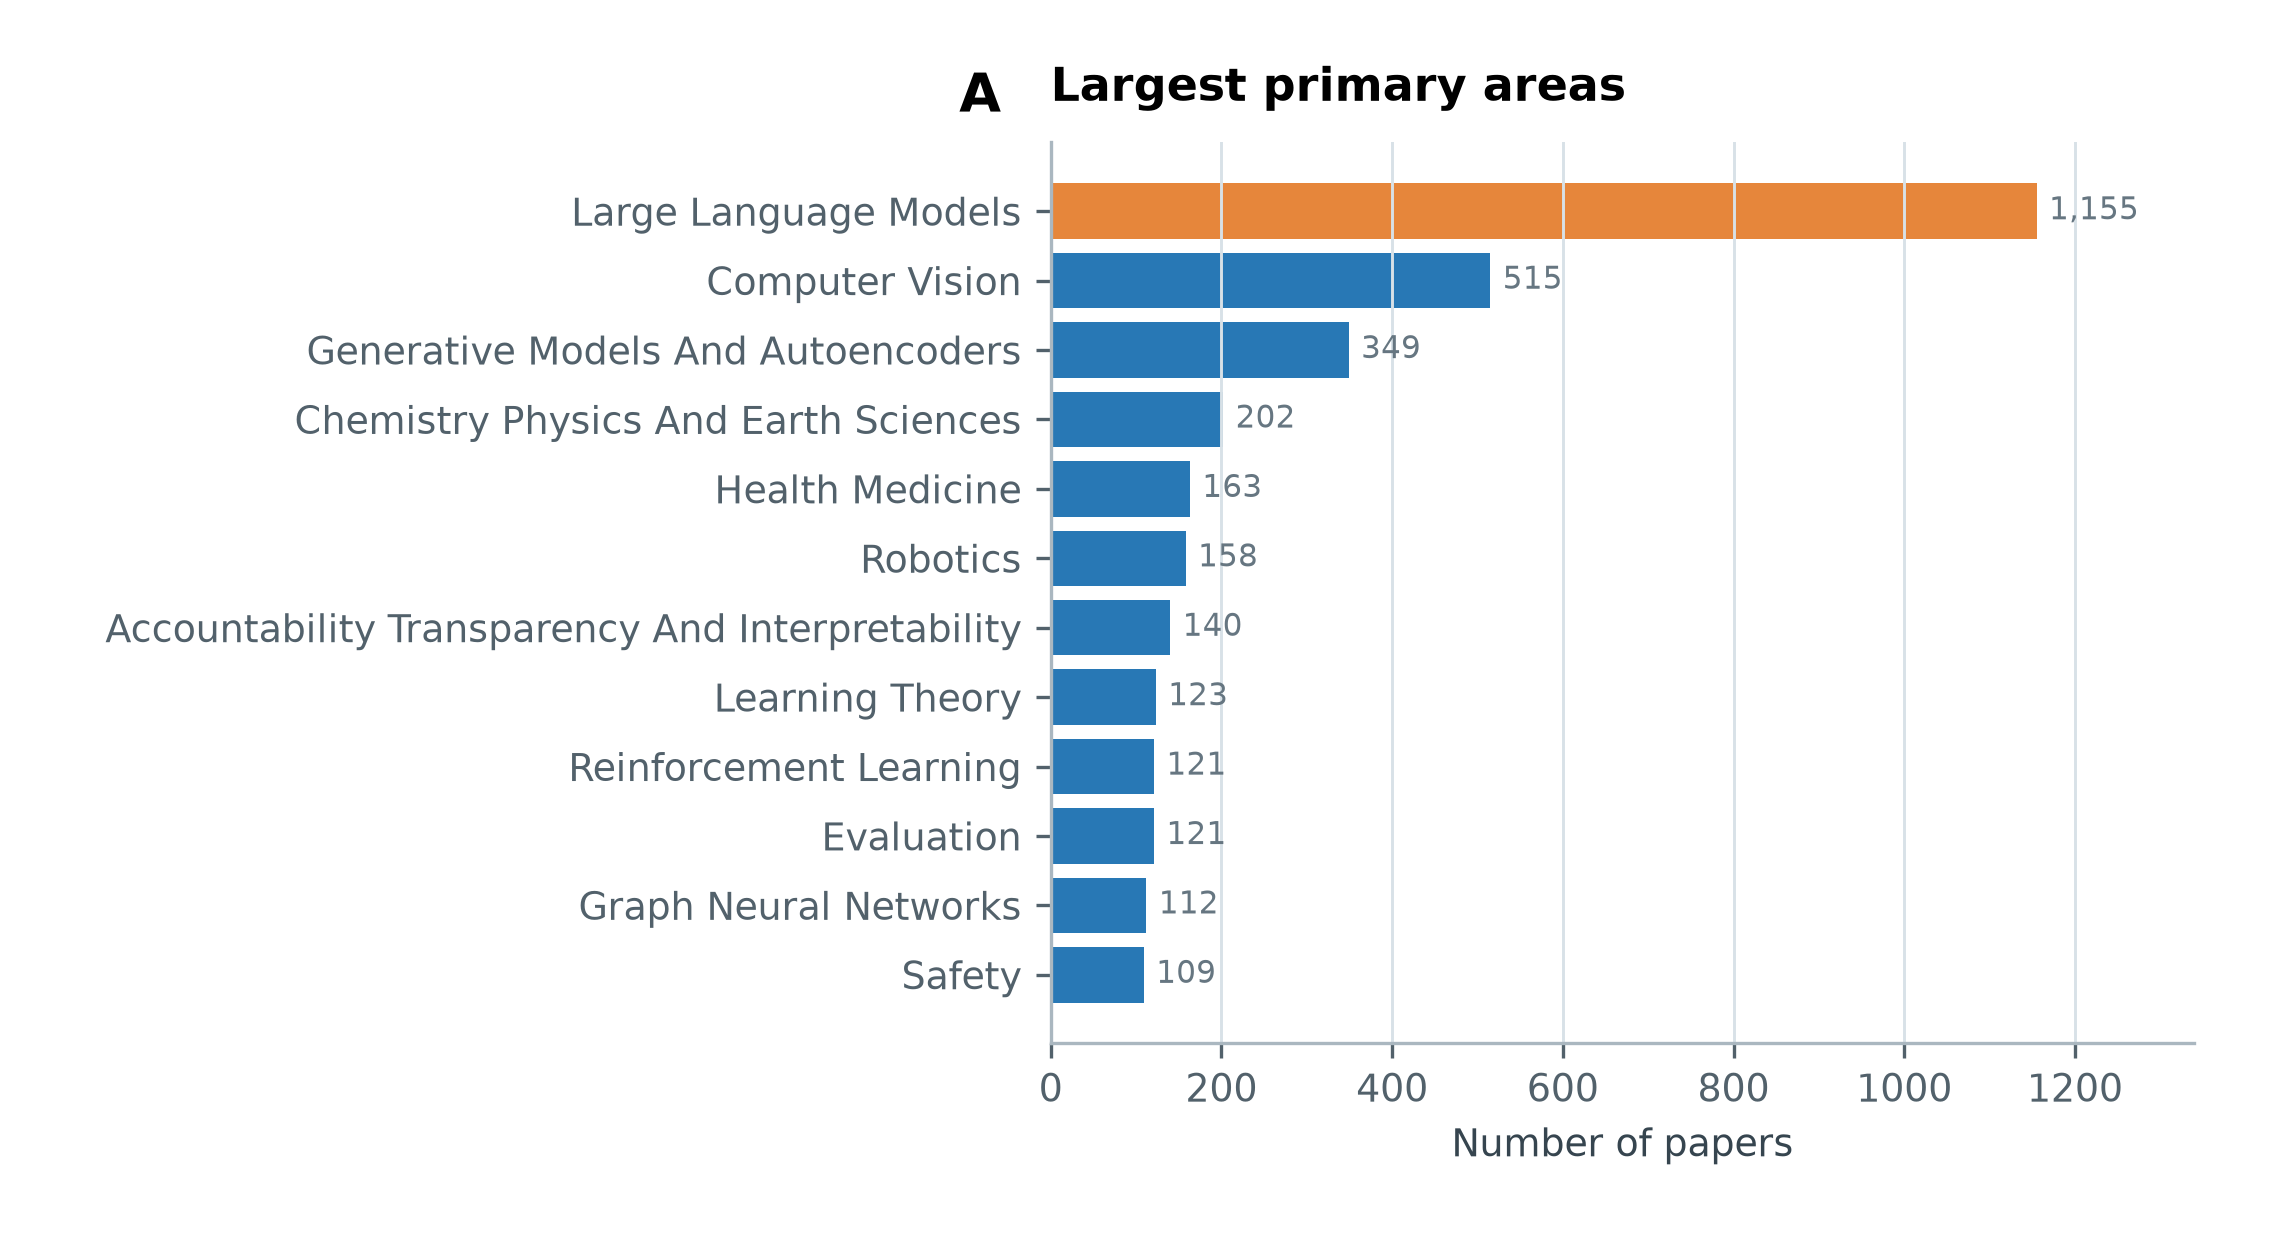
\includegraphics[width=\textwidth]{../psudo_labeling/figure/icml2026/individual/01_primary_area_distribution.png}
  \end{subfigure}\hfill
  \begin{subfigure}[t]{0.36\textwidth}
    \centering
    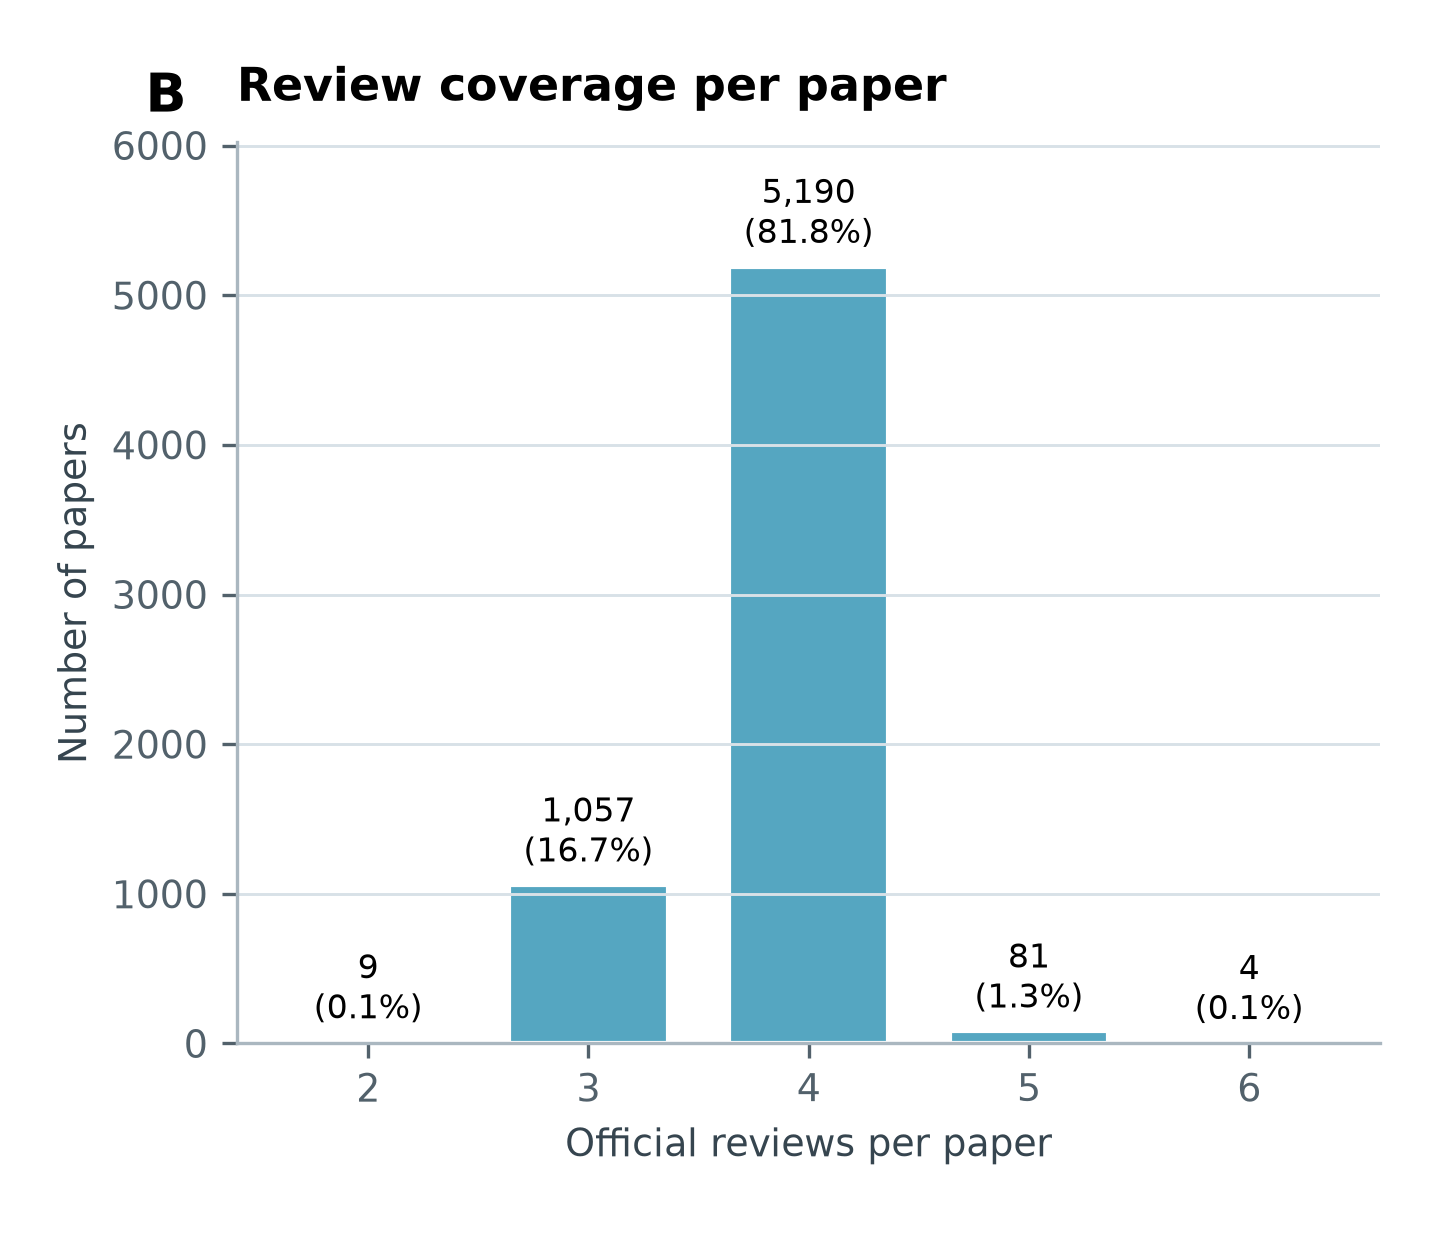
\includegraphics[width=\textwidth]{../psudo_labeling/figure/icml2026/individual/02_reviews_per_paper.png}
  \end{subfigure}
  \caption{Population coverage. Large Language Models is the largest primary area (1,155 papers), followed by Computer Vision (515) and Generative Models and Autoencoders (349). Most papers have four official reviews (5,190 papers; 81.8\%), while 16.7\% have three.}
  \label{fig:population-coverage}
\end{figure*}

\begin{figure*}[p]
  \centering
  \begin{subfigure}[t]{0.54\textwidth}
    \centering
    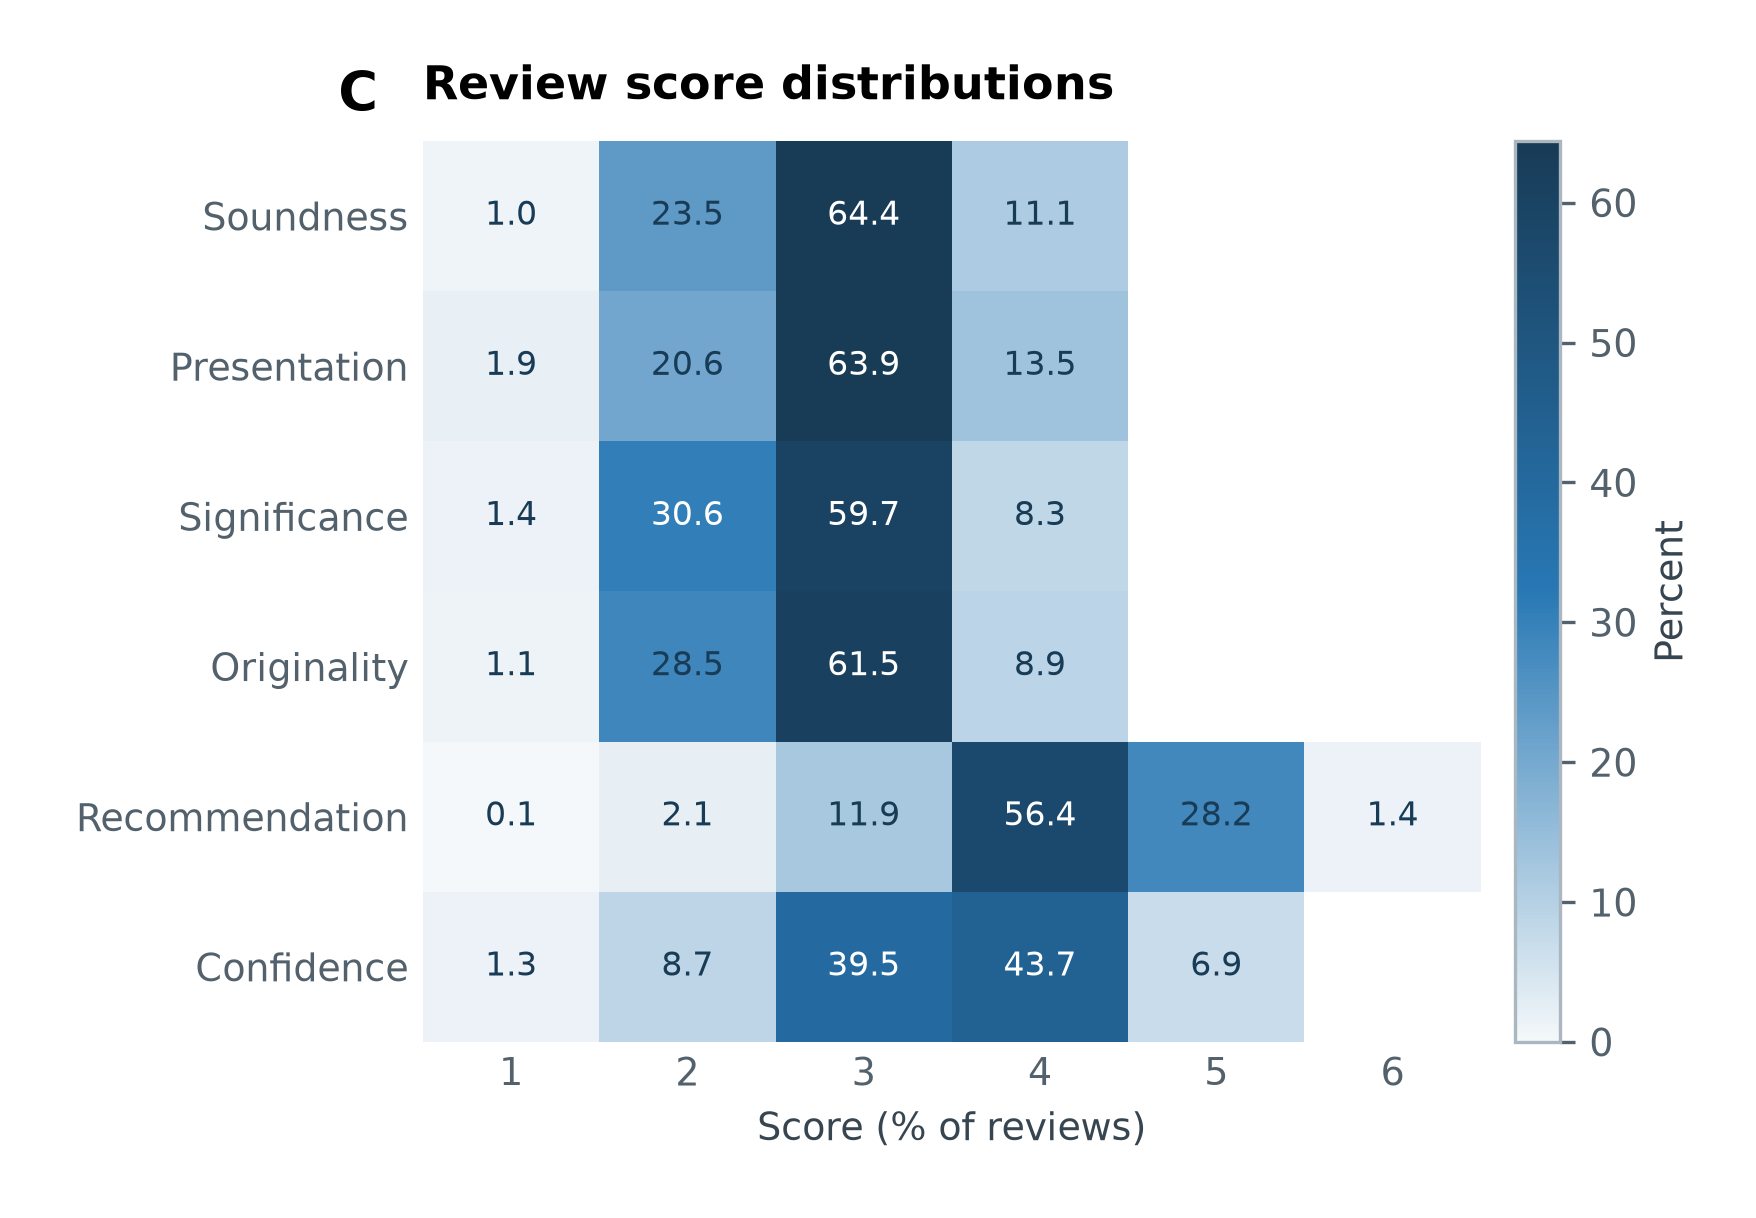
\includegraphics[width=\textwidth]{../psudo_labeling/figure/icml2026/individual/03_review_score_distributions.png}
  \end{subfigure}\hfill
  \begin{subfigure}[t]{0.42\textwidth}
    \centering
    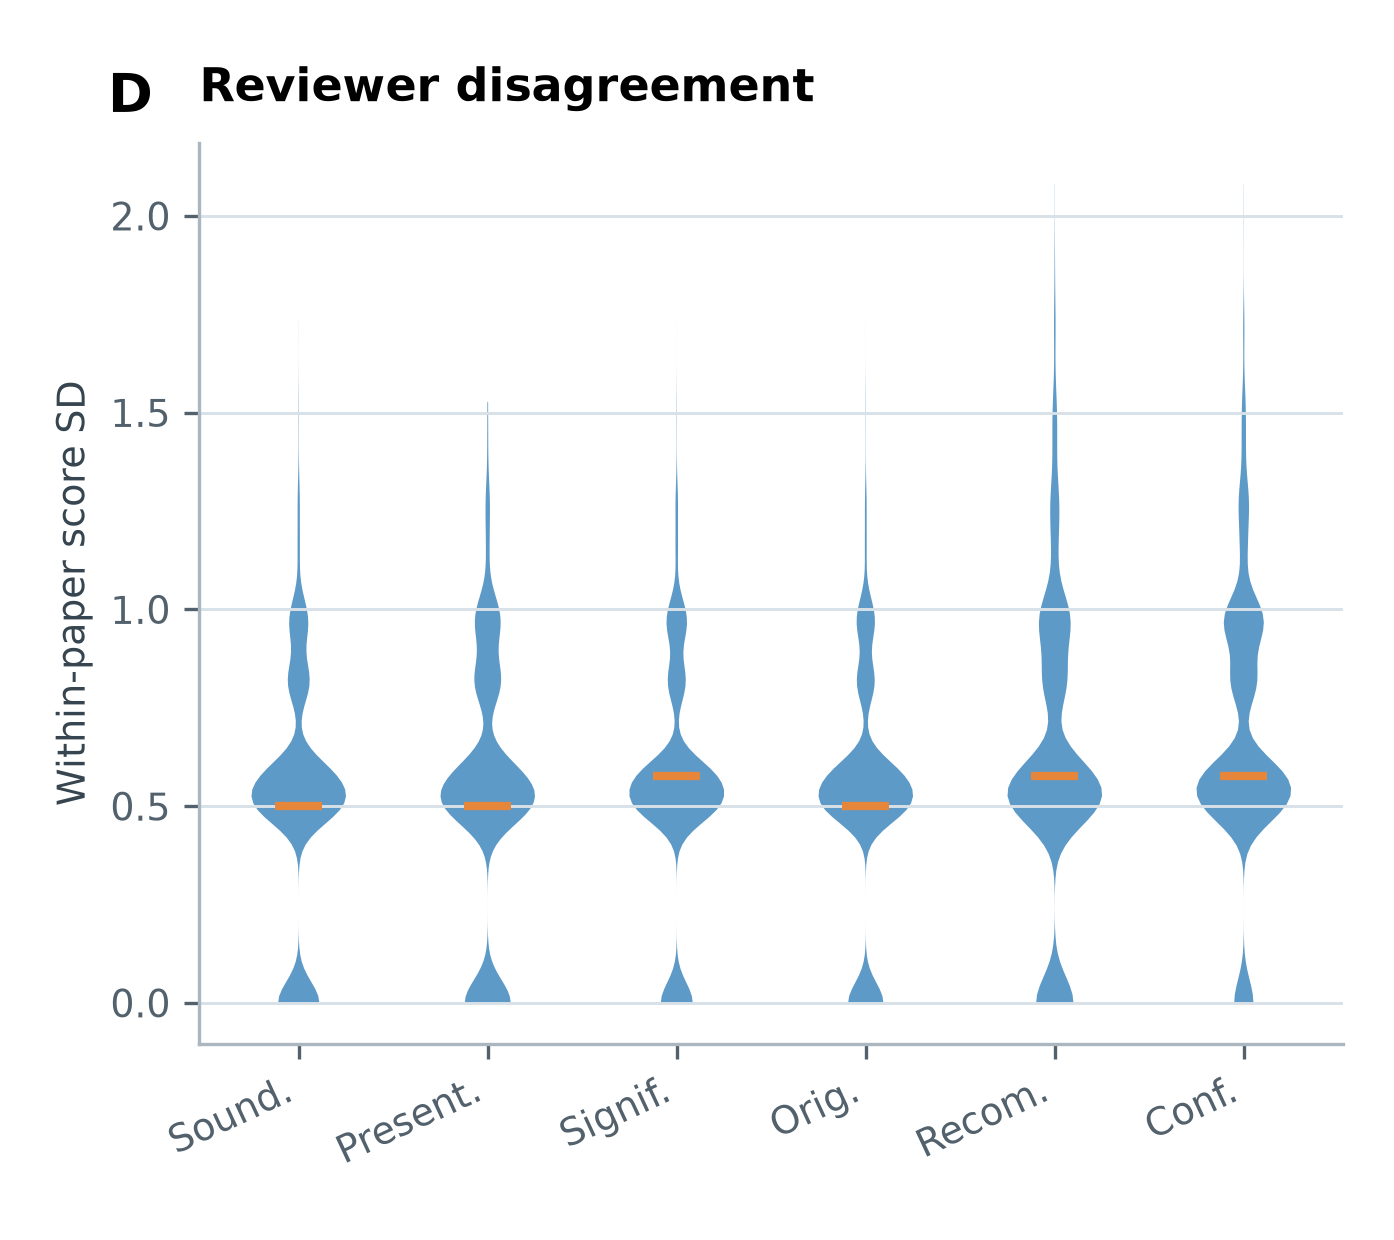
\includegraphics[width=\textwidth]{../psudo_labeling/figure/icml2026/individual/04_reviewer_disagreement.png}
  \end{subfigure}
  \caption{Human-review scores and within-paper disagreement. Scores concentrate at 3 for the four quality dimensions and at 4 for overall recommendation; confidence is concentrated at 3--4. The violin plots show the standard deviation across reviewers for each paper. Median disagreement is approximately 0.5 points for all six dimensions, with substantial upper tails. This variation motivates consolidating multiple reviews rather than treating an arbitrary individual review as the supervision target.}
  \label{fig:human-score-statistics}
\end{figure*}

\begin{figure*}[p]
  \centering
  \begin{subfigure}[t]{0.60\textwidth}
    \centering
    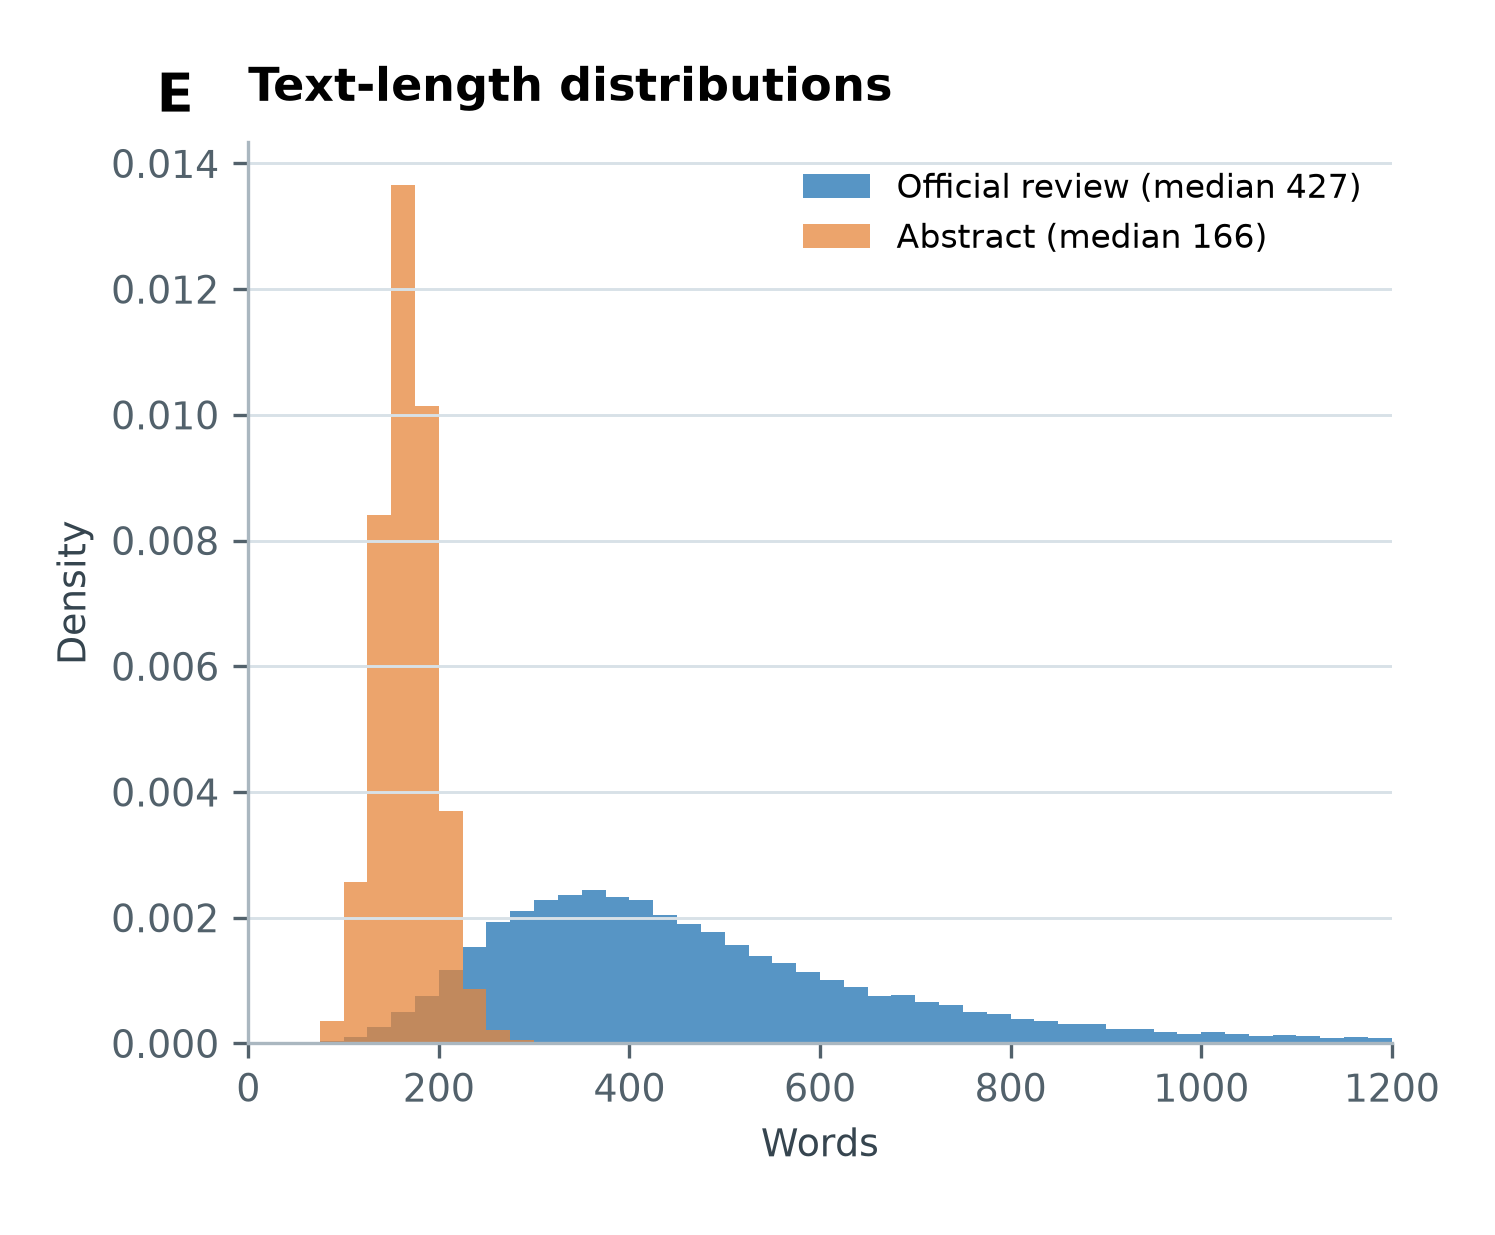
\includegraphics[width=\textwidth]{../psudo_labeling/figure/icml2026/individual/05_text_length_distributions.png}
  \end{subfigure}\hfill
  \begin{subfigure}[t]{0.34\textwidth}
    \centering
    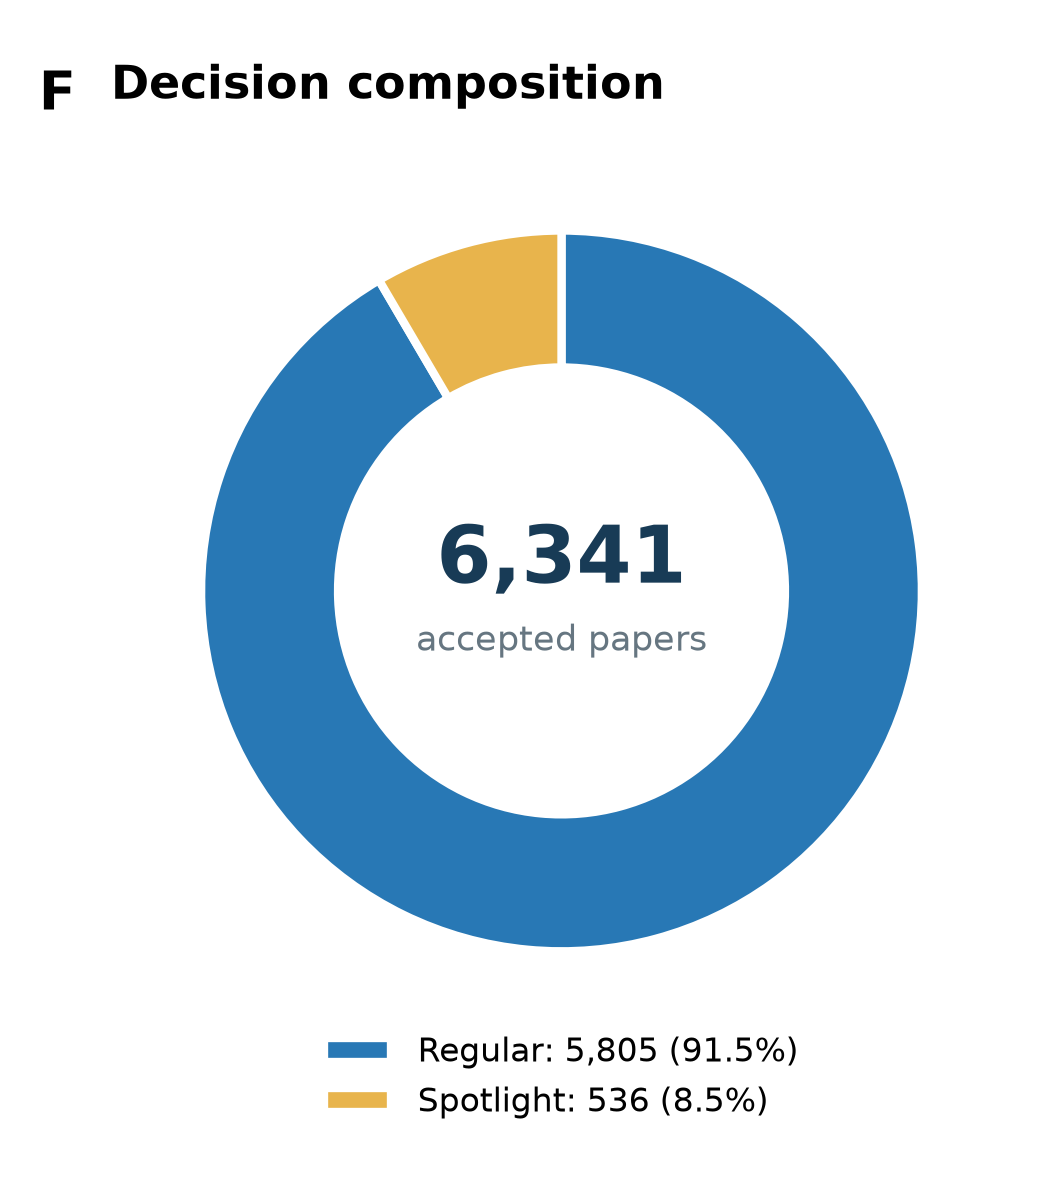
\includegraphics[width=\textwidth]{../psudo_labeling/figure/icml2026/individual/06_decision_composition.png}
  \end{subfigure}
  \caption{Text length and decision composition of the accepted-paper population. Official reviews have a median length of 427 words, compared with 166 words for abstracts, and exhibit a much longer right tail. The population contains 5,805 regular papers (91.5\%) and 536 spotlight papers (8.5\%).}
  \label{fig:text-decision-statistics}
\end{figure*}

\subsection{Pseudo-label score comparison}
We compare three quantities for each score dimension: the distribution of paper-level mean human scores over all 6,341 papers, the same statistic for the 175 papers with completed pseudo-labels, and the single consolidated score assigned to each of those 175 papers. Human scores are averaged within a paper before aggregation so that papers with more reviews do not receive greater weight. Mean comparisons use 95\% normal intervals. This analysis is descriptive: the 175-paper set is an intermediate labeled subset, not a held-out evaluation sample.

\begin{figure*}[p]
  \centering
  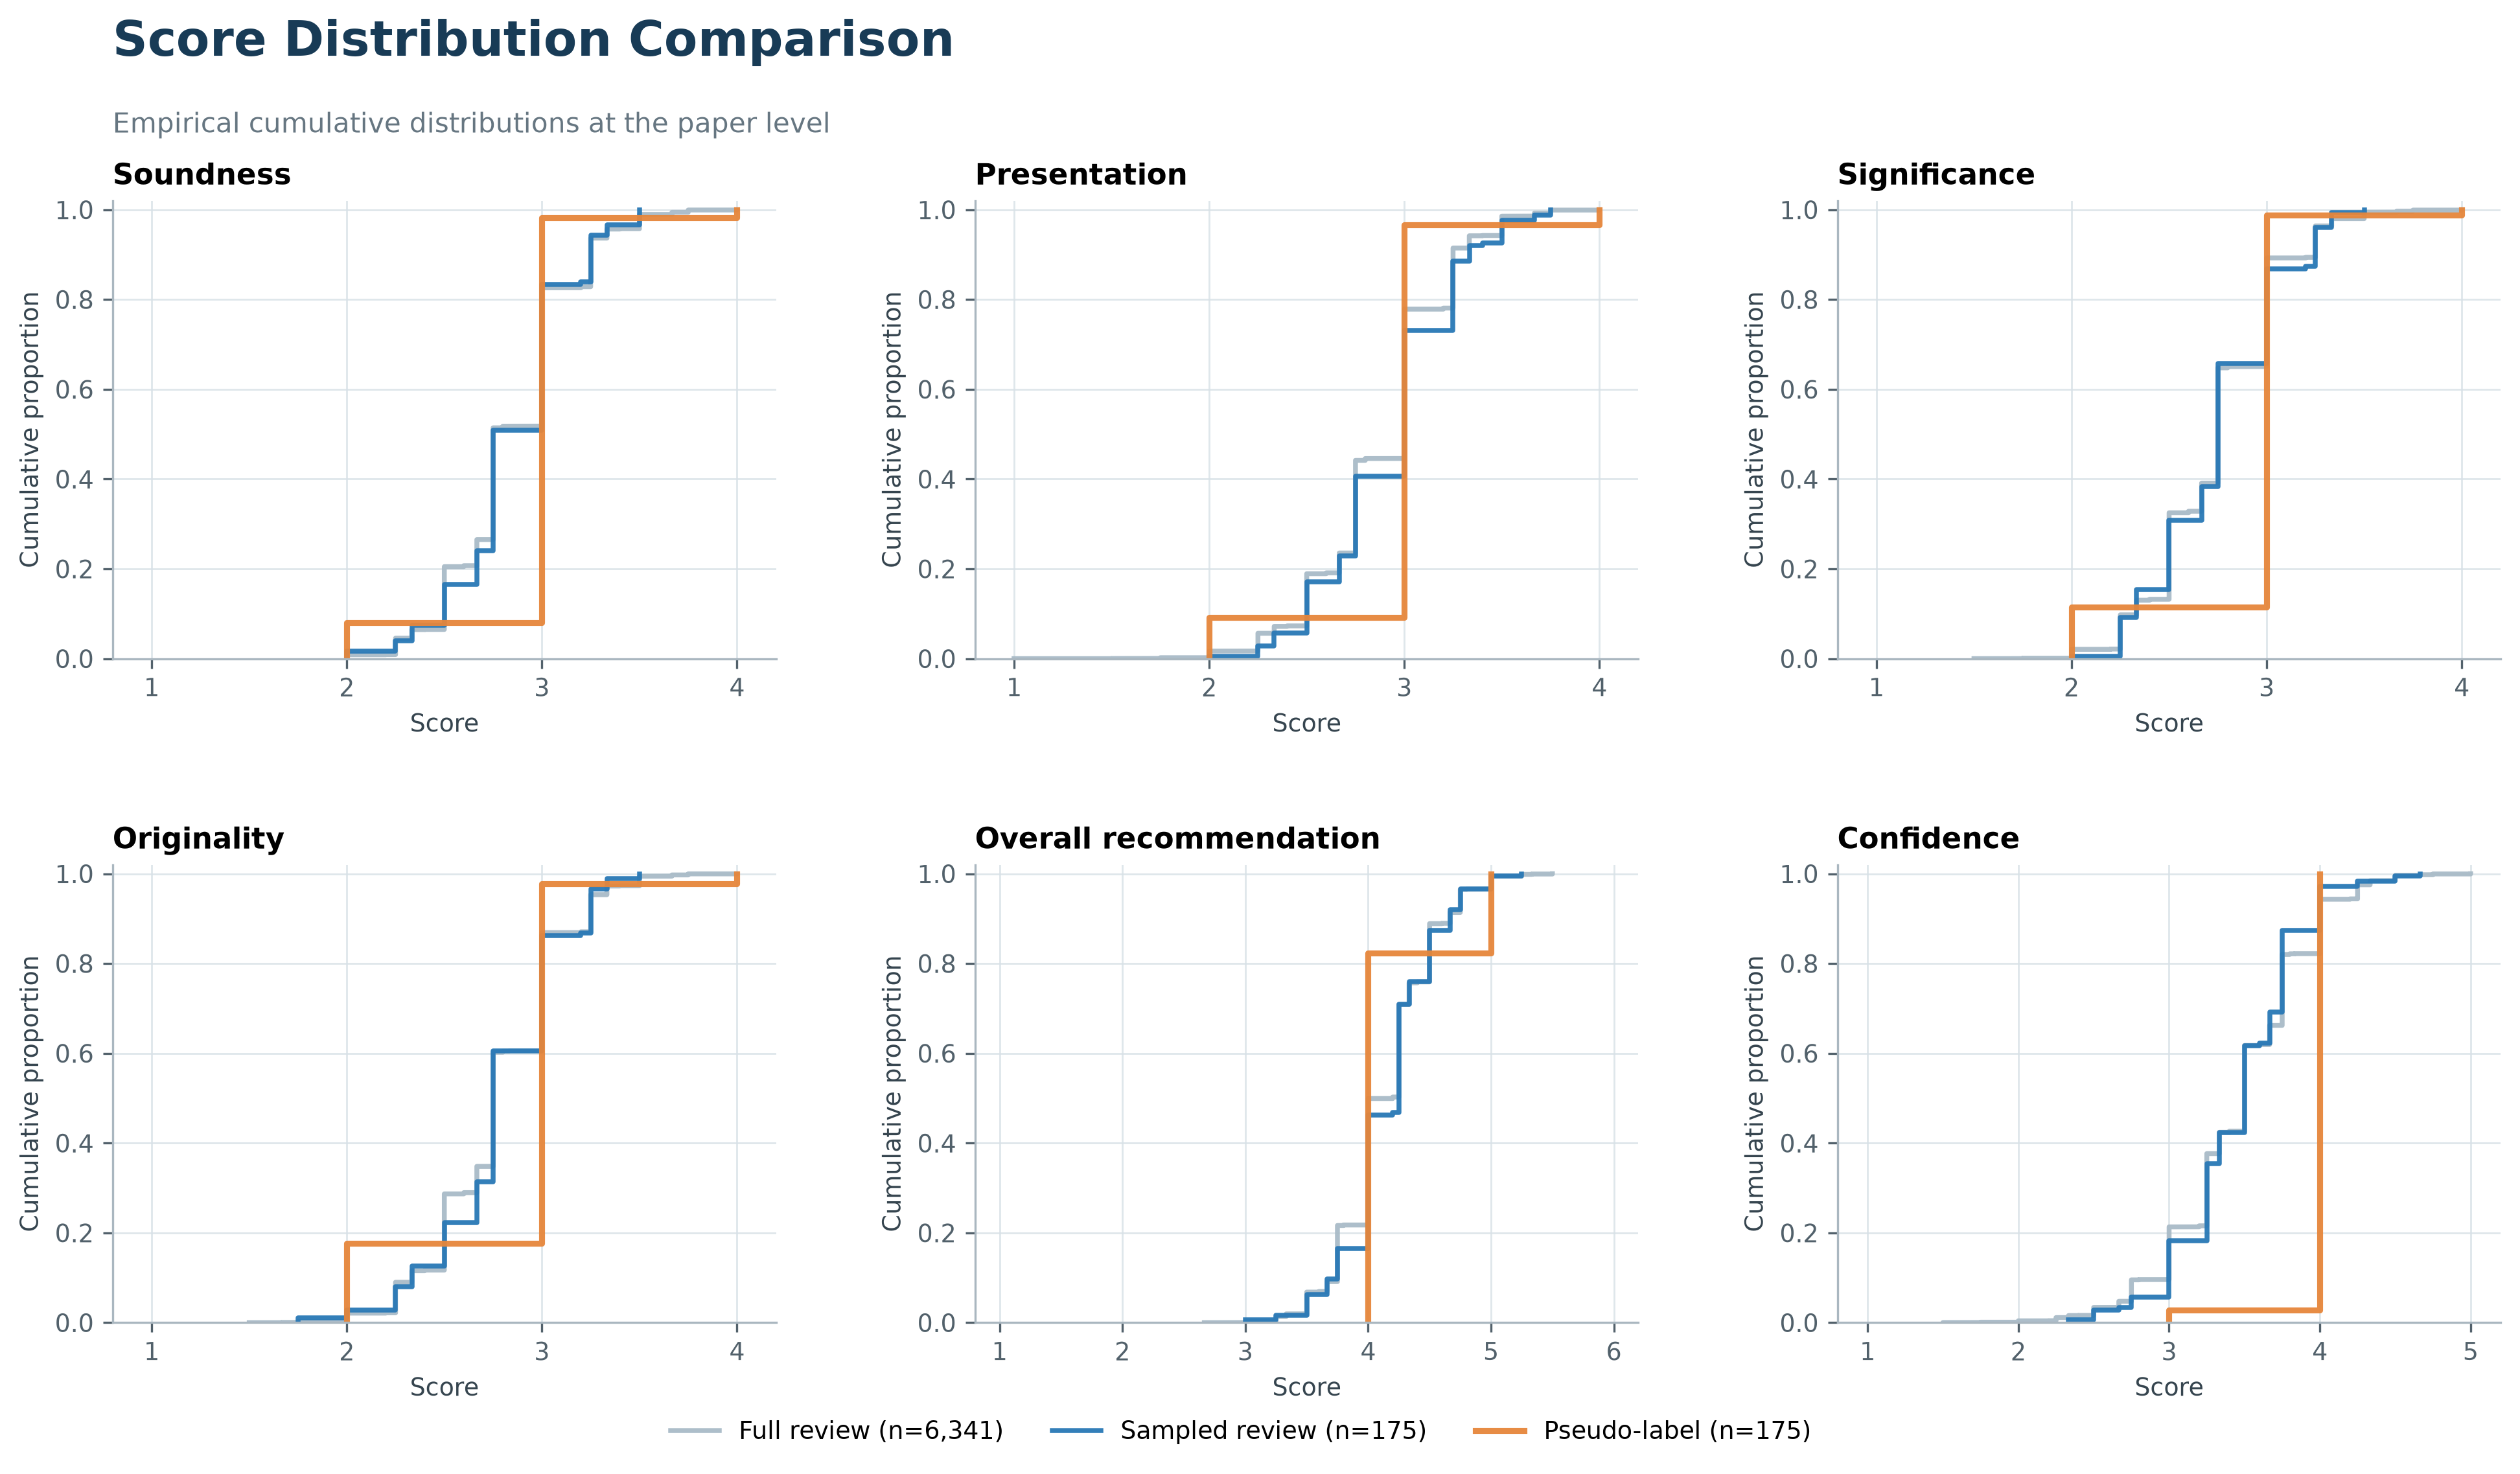
\includegraphics[width=0.96\textwidth]{../psudo_labeling/figure/icml2026/pseudo_score_comparison/score_distributions_comparison.png}
  \caption{Empirical cumulative score distributions for the full accepted-paper population, the 175-paper labeled subset, and its consolidated pseudo-labels. The full and sampled human curves are similar. Pseudo-label curves have larger jumps because each paper receives one integer label, whereas the human curves use fractional within-paper averages. Consolidated quality scores also concentrate near 3, overall recommendation near 4, and confidence near 4.}
  \label{fig:pseudo-score-distributions}
\end{figure*}

\begin{figure*}[p]
  \centering
  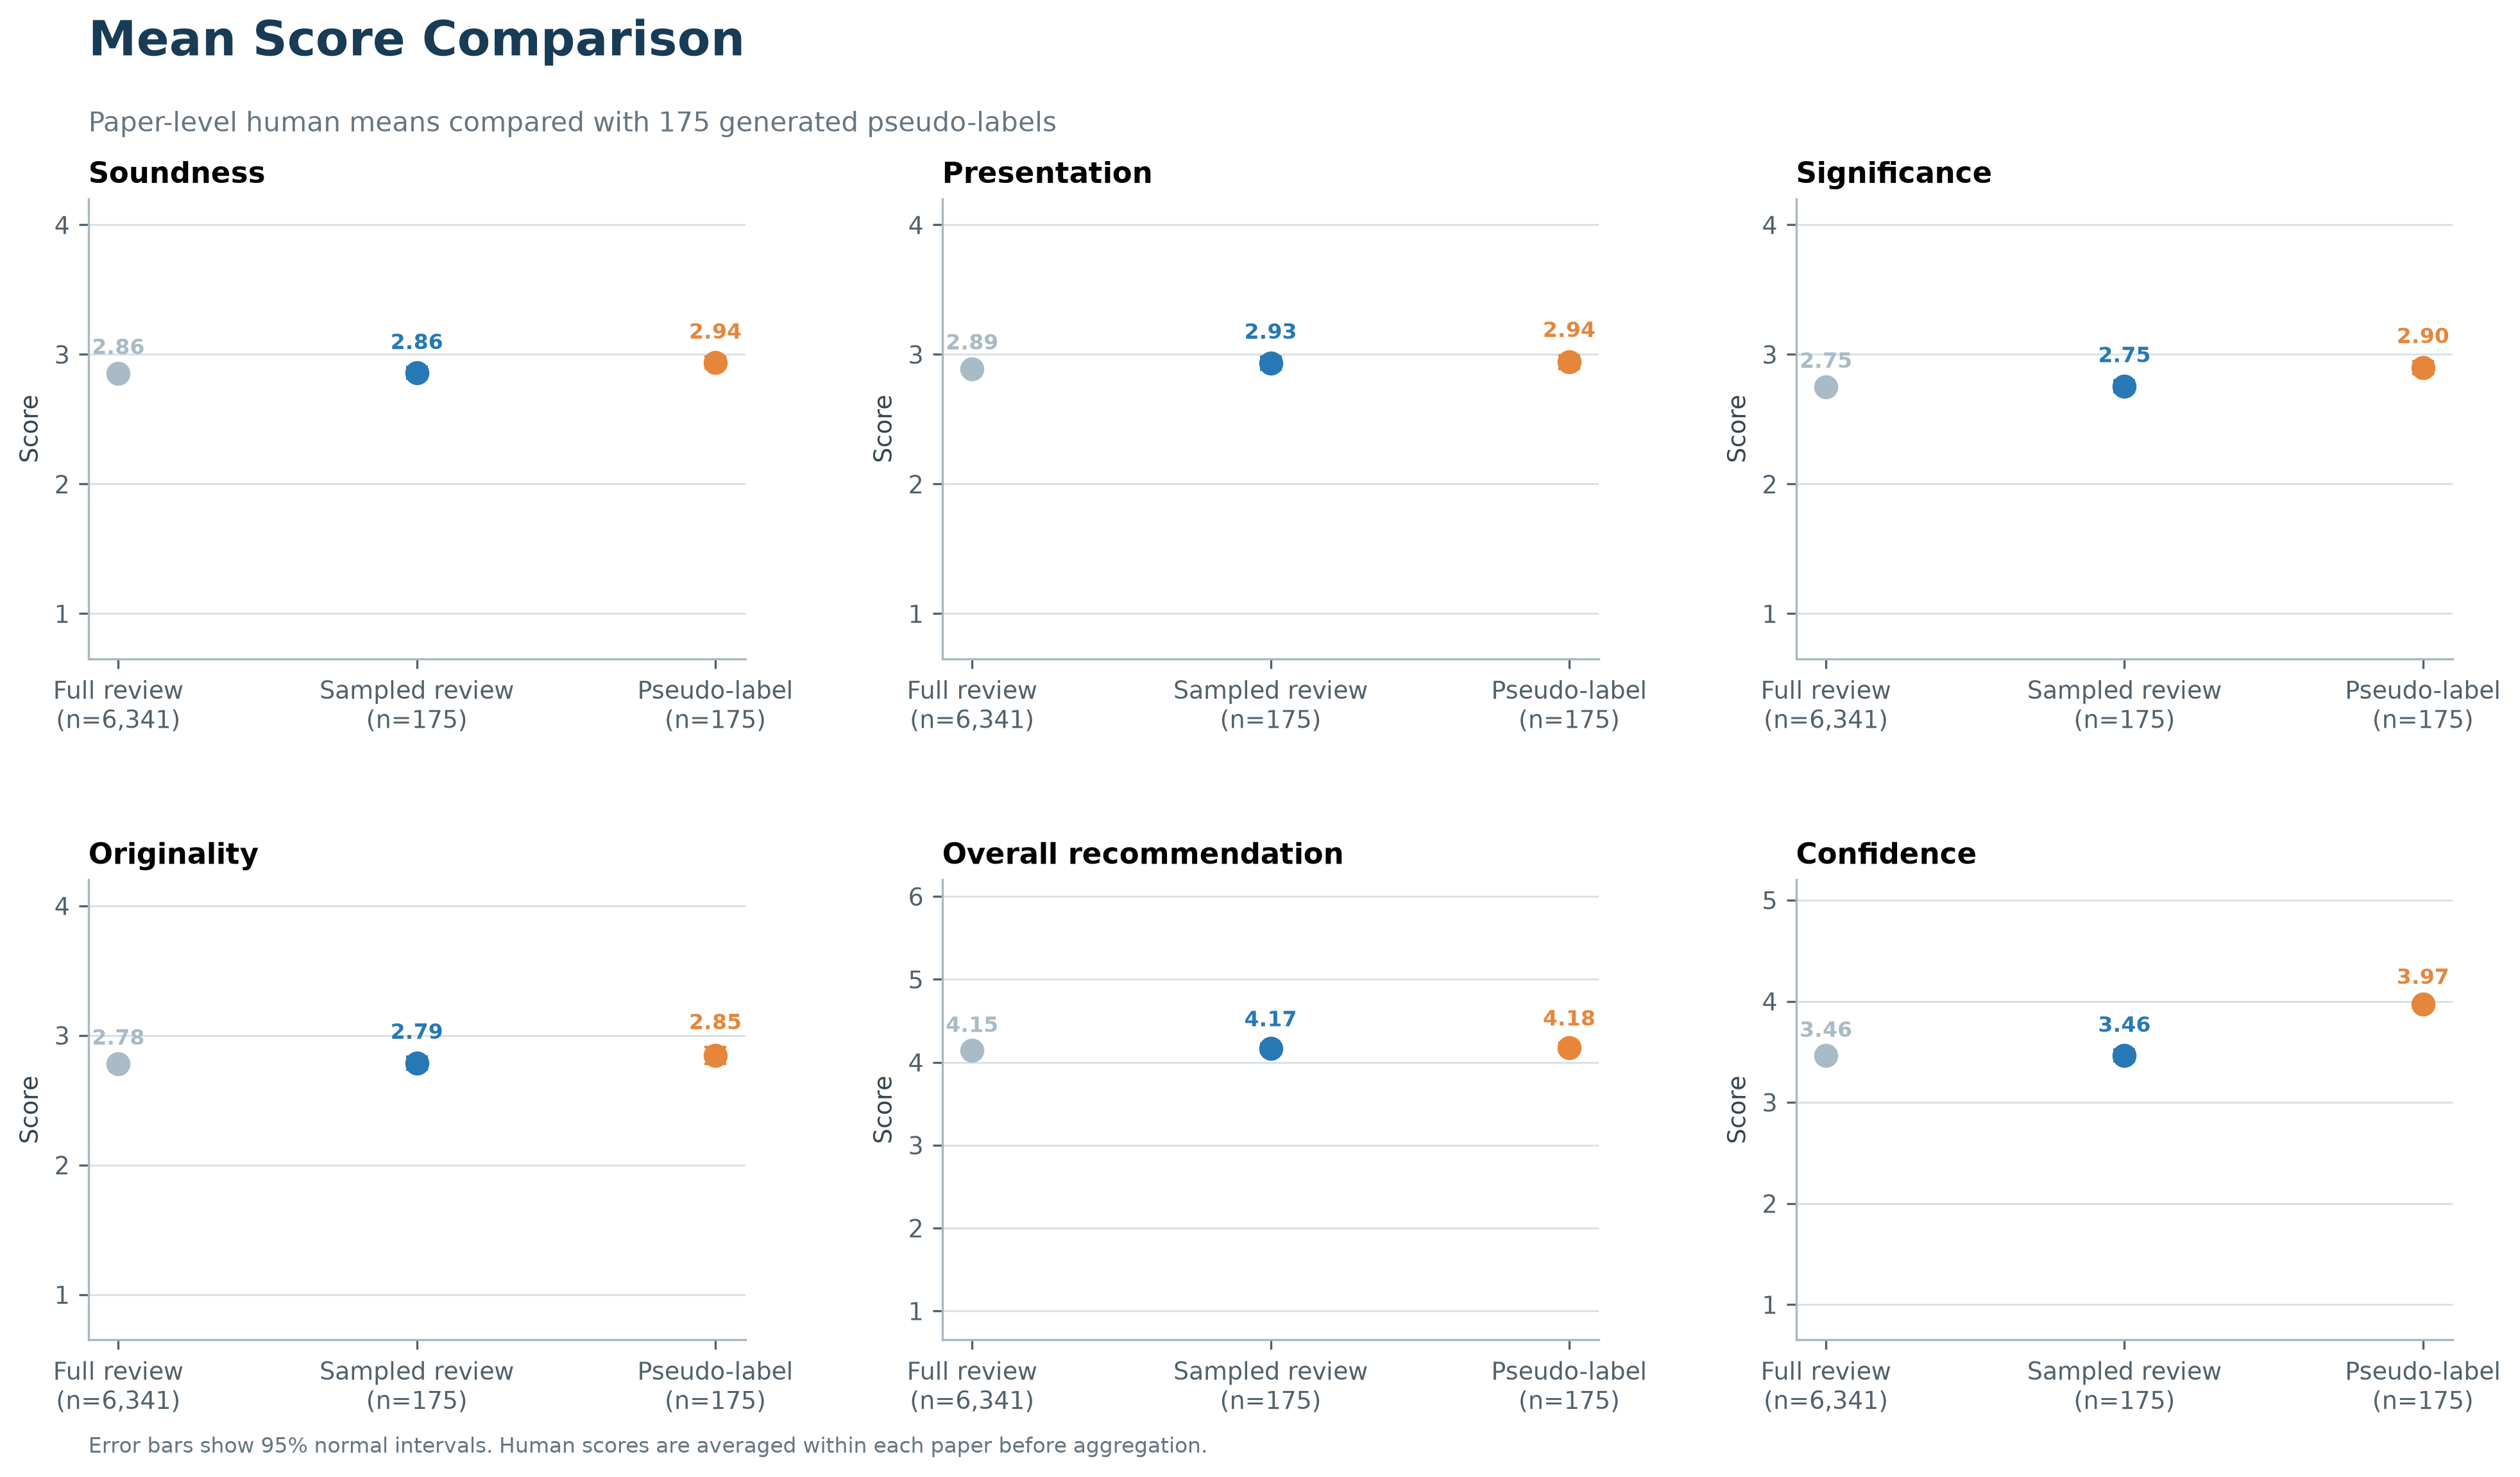
\includegraphics[width=0.96\textwidth]{../psudo_labeling/figure/icml2026/pseudo_score_comparison/score_means_comparison.png}
  \caption{Mean score comparison with 95\% normal intervals. For the full population, sampled human reviews, and pseudo-labels, respectively, the means are 2.86/2.86/2.94 for soundness, 2.89/2.93/2.94 for presentation, 2.75/2.75/2.90 for significance, 2.78/2.79/2.85 for originality, and 4.15/4.17/4.18 for overall recommendation. Confidence increases from 3.46 in both human sets to 3.97 in the pseudo-labels, indicating that the consolidation procedure produces more decisive confidence judgments than a paper-level mean of reviewer confidence.}
  \label{fig:pseudo-score-means}
\end{figure*}

Together, \Cref{fig:pseudo-score-distributions,fig:pseudo-score-means} show that consolidation broadly preserves central score tendencies but is not distribution-neutral. In particular, converting several reviews into one ordinal target removes within-paper averaging and shifts confidence upward. We therefore retain reviewer-level scores and label-audit metadata for downstream diagnostics rather than interpreting pseudo-labels as literal human consensus.

\begin{figure*}[t]
  \centering
  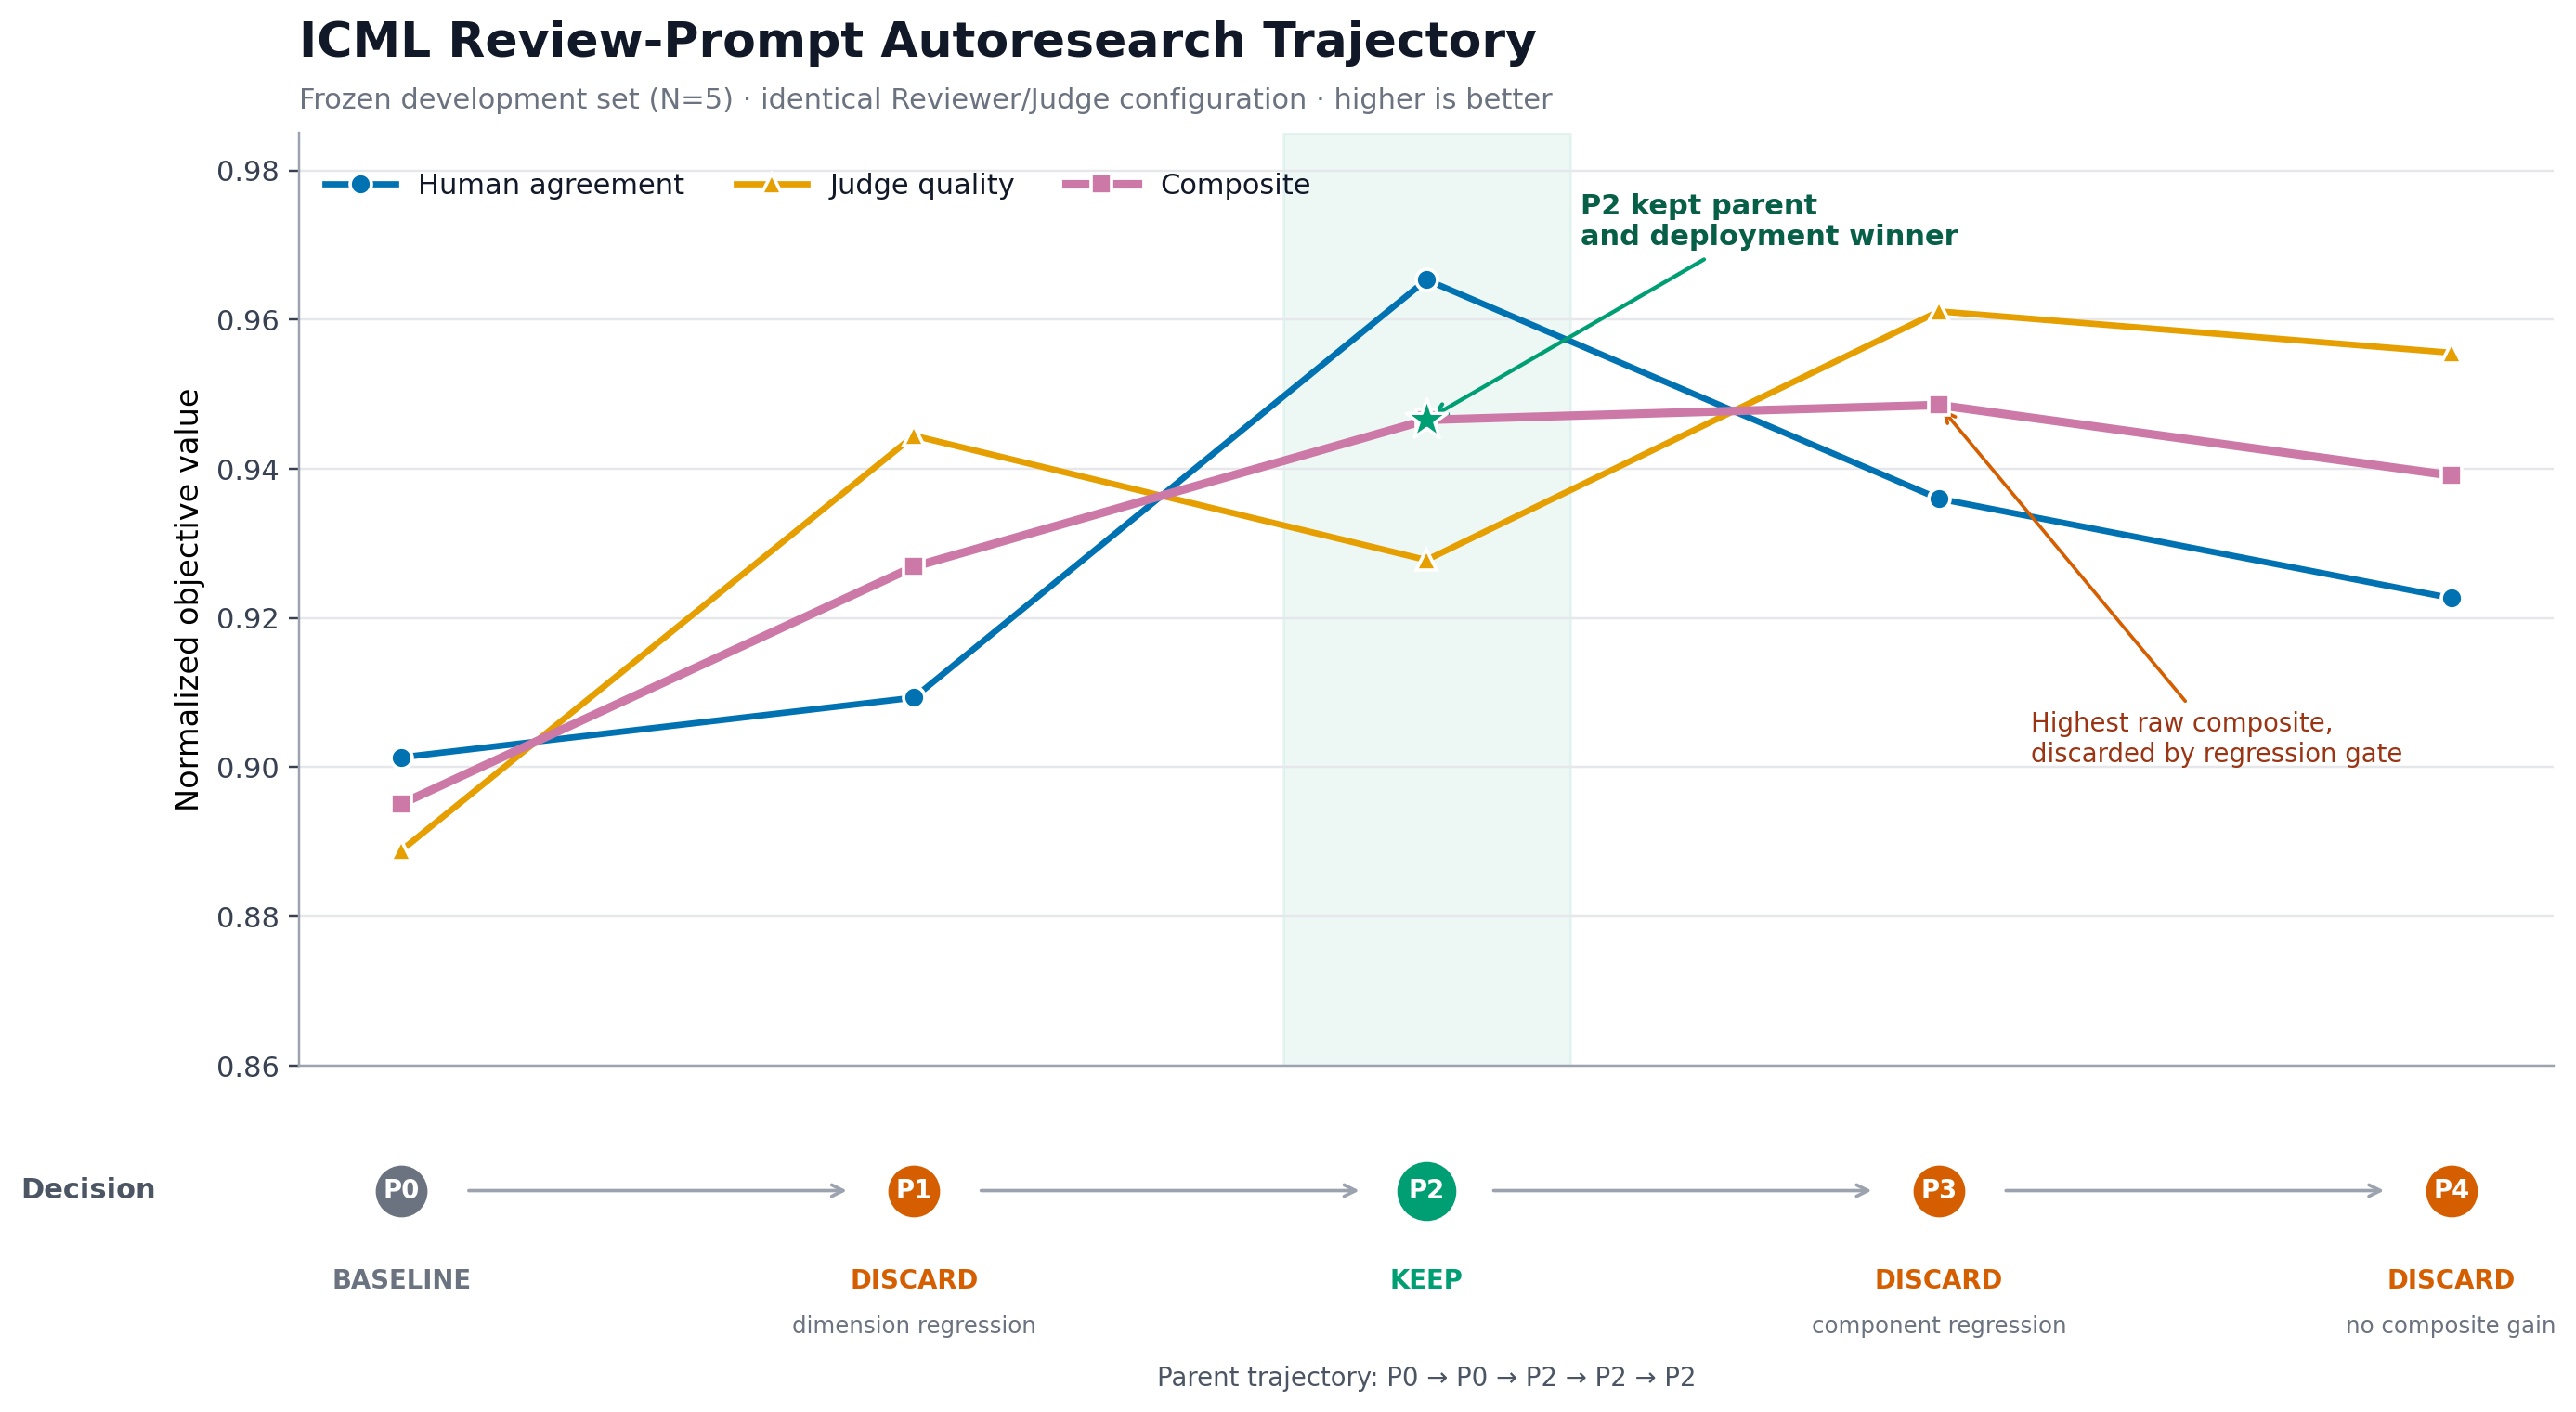
\includegraphics[width=0.96\textwidth]{../docs/figures/review-prompt-autoresearch-trajectory.png}
  \caption{Prompt-optimization trajectory on the frozen five-paper development set. P2 is retained because it improves the composite objective and passes all component and dimension regression gates; P1, P3, and P4 are discarded.}
  \label{fig:trajectory}
\end{figure*}

\section{Review-Agent Implementation}
\paragraph{Reviewer configuration.}
The final agent combines the P2 instructions selected by the five-paper development campaign with GPT-5.4 as the reviewer model. The prompt asks the model to first identify the paper's principal claims and supporting evidence, then evaluate weaknesses by severity, and finally calibrate the ordinal scores against the written assessment. The model and prompt are held fixed for all reported runs. P2 should be interpreted only as the winner of this bounded development campaign, rather than as a universally optimal reviewer.

\paragraph{Input isolation and reviewer invocation.}
Each input PDF is converted to plain text and placed in a delimited untrusted-data block following the fixed reviewer instructions. The extracted text is used only for the inference call. Reviewer inference has no access to shell tools, external applications, subagents, persistent memory, plugins, or web search. The request contains neither human reviews nor consolidated labels, reference scores, Judge feedback, candidate identities, or optimization traces. Consequently, the agent is label-blind and bases its assessment only on the supplied manuscript.

\paragraph{Structured generation and validation.}
The model returns a single structured review containing a summary; lists of strengths, weaknesses, and author questions; limitations; ethical concerns; an evidence trace; six ordinal scores; and a rationale for every score. The four quality dimensions use the 1--4 ICML scale, overall recommendation uses 1--6, and confidence uses 1--5. The JSON schema forbids unknown fields and requires all sections. A second runtime validator checks types, nonempty prose and lists, the exact score keys, and every numerical range. Invalid output or a transient inference failure may trigger at most one retry; persistent failure produces no completed review.

\paragraph{Review representation and auditability.}
Each successful inference yields one machine-readable assessment and an equivalent human-readable rendering. Both representations contain the same review content: claim summary, strengths, severity-ordered weaknesses, questions for the authors, limitations, ethical concerns, evidence trace, scores, and score rationales. For experimental audit, we retain the model and prompt version, input identity, token usage, retry count, and schema-validation outcome. Manuscript text, human reviews, pseudo-labels, and Judge feedback are excluded from the agent output. This separation allows a generated assessment to be traced to a fixed experimental condition without exposing evaluator-only supervision to the reviewer.

\end{document}
